\begin{wrapfigure}[9]{r}{0.55\linewidth}
    \centering
    \vspace{-6mm}
    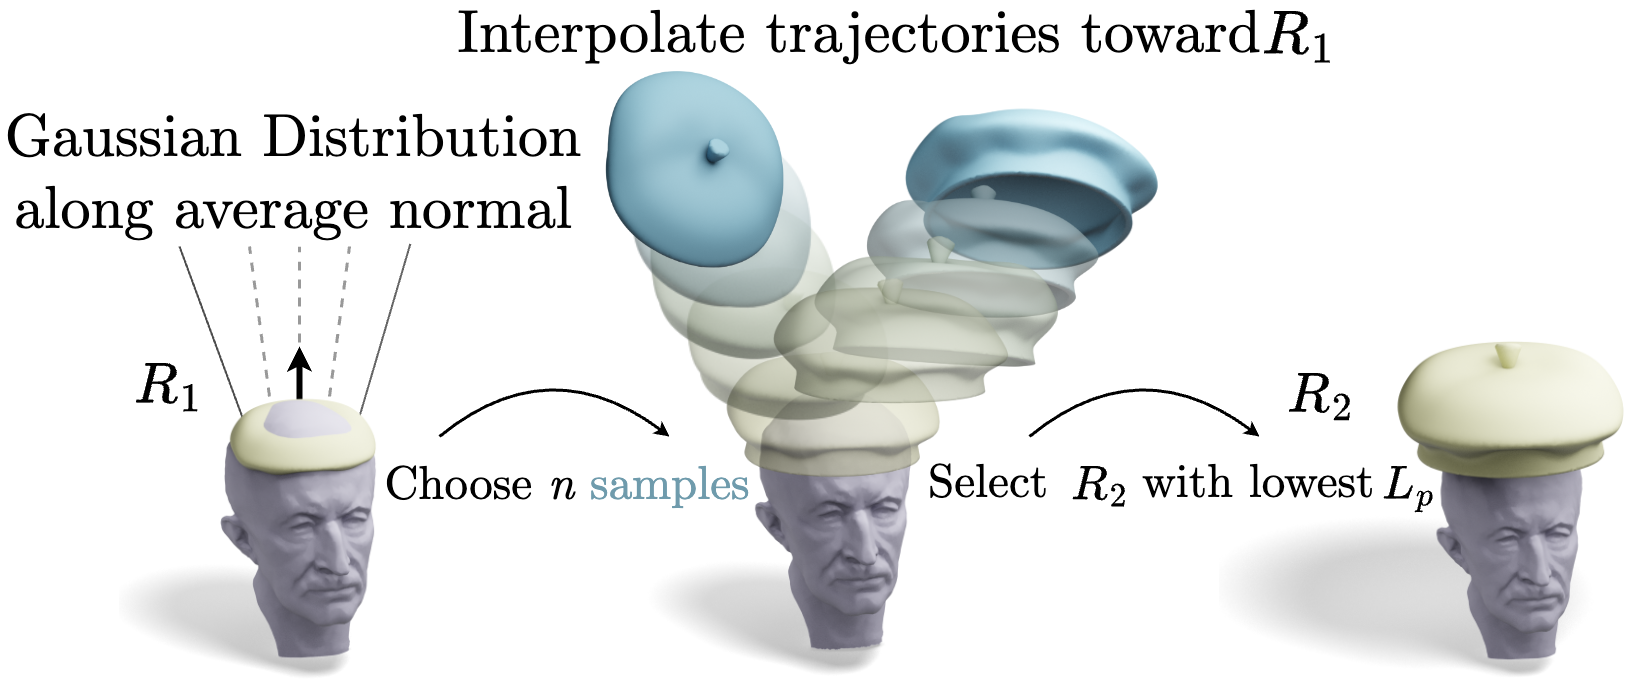
\includegraphics[width=\linewidth]{figures/trajectory_method/trajectory_method.png}
    \caption{}
    % \caption{To find a non-intersecting configuration, we simulate several possible object trajectories and sample different timesteps (see \autoref{sec:step2}). Among all non-intersecting candidates, we select the one closest to the target region of the base mesh.}
    \label{fig:trajectory_method}
\end{wrapfigure}